\graphicspath{{chapters/software/}}
\chapter{CCA-Zoo: A collection of Regularized, Deep Learning-based, Kernel, and Probabilistic methods in a scikit-learn style framework}\label{ch:ccazoo}

% \epigraph{What I mean is that if you really want to understand something, the best way is to try and explain it to someone else. That forces you to sort it out in your mind. And the more slow and dim-witted your pupil, the more you have to break things down into more and more simple ideas. And that's really the essence of programming. By the time you've sorted out a complicated idea into little steps that even a stupid machine can deal with, you've learned something about it yourself.}{\textit{Douglas Adams}}

\section{Introduction}

The Python programming language has seen a surge in popularity in the machine learning community due to its versatility and extensive libraries.
However, when it comes to the domain of multiview learning, there is a noticeable void in the Python ecosystem.
Existing libraries, such as \texttt{scikit-learn}\cite{pedregosa2011scikit}, offer basic implementations for Canonical Correlation Analysis (CCA) and Partial Least Squares (PLS), yet fall short of providing a comprehensive toolkit for multiview learning techniques.
This is particularly striking given the widespread recognition that the availability of quality software implementations often acts as a catalyst for the adoption of novel methodologies in the statistical learning community.

One glaring example of this trend is Sparse PLS. Despite its known limitations, Sparse PLS has effectively become the go-to method for sparse CCA applications, primarily due to its robust implementation in the R programming language.
The discrepancy between the availability of multiview learning tools in R and Python has not only hindered the diversification of methodologies but also impeded the community from leveraging the more recent advances in the field.

\section{Background}

In recent years, the research community has shown a heightened interest in multiview learning, as evident from the proliferation of scholarly articles and the diversification of use-cases ranging from bioinformatics to natural language processing.
Traditionally, this field has been dominated by contributions from statistical learning researchers who predominantly utilized R and MATLAB for their work.
These platforms have been the birthplace of many state-of-the-art algorithms and methodologies, including but not limited to Sparse PLS.

However, this posed a challenge for Python-oriented researchers and practitioners, leaving them with two less-than-ideal options: either port existing R or MATLAB code into Python, often a non-trivial task requiring domain expertise, or resort to using the limited set of methods available in native Python libraries like \texttt{scikit-learn}.
This fragmentation has, in effect, created barriers to entry and possibly slowed down the progress in applying multiview learning techniques in Python-based projects.

The \texttt{CCA-Zoo} package aims to bridge this divide by offering a broad range of multiview learning algorithms, creating a unified platform that fosters both academic research and practical applications in Python.

\section{Methods}

In this section, we describe the implementation of \texttt{CCA-Zoo} and the design decisions that were made during its development.
We will also demonstrate how the package is optimised for use with high-dimensional biomedical data.

\subsection{API}

The \texttt{scikit-learn} API is familiar to many machine learning practitioners and researchers, and is the de facto standard for machine learning in Python.
Users of machine learning libraries in Python expect a consistent API, and so we have designed \texttt{CCA-Zoo} to be compatible with the \texttt{scikit-learn} API.
Moreover, by using the \texttt{scikit-learn} API, \texttt{CCA-Zoo} is compatible with the \texttt{scikit-learn} ecosystem.

The major barrier to using the \texttt{scikit-learn} API for multiview learning is that the \texttt{scikit-learn} API is designed for single-view data.
In particular, the \texttt{scikit-learn} API for fitting a model is \texttt{model.fit(X, y)}, where \texttt{model} is an instance of a model, \texttt{X} is a matrix of features, and \texttt{y} is a vector of labels.

In multiview learning, we have multiple views of data \texttt{X}, and so we need to be able to fit a model with multiple views of data.
For this reason, models in \texttt{CCA-Zoo} have a \texttt{fit} method that takes a list of views as input, i.e. \texttt{model.fit([X1, X2, X3], y)}.

\subsection{Models}

\subsubsection{Linear Models}

\subsubsection{Deep Models}


\subsubsection{Model Selection}

Model selection and cross-validation are crucial steps to all of the models described in this thesis and in particular models with hyperparameters.
In this section, we describe the model selection API in \texttt{CCA-Zoo} and how it is optimised for use with high-dimensional biomedical data.

\subsubsection{Grid Search}

In order to be compatible with the

\subsubsection{Random Search}

\subsubsection{Visualisation}

\section{Benchmarking}

\subsubsection{Objective}
The objective of the benchmarking experiments is to compare the performance of \texttt{CCA-Zoo} against \texttt{scikit-learn}, focusing on the efficiency of Canonical Correlation Analysis (CCA) and Partial Least Squares (PLS) methods.
We conducted experiments on synthetic datasets with varying dimensions to evaluate their average execution time.

\subsubsection{Experimental Setup}
The datasets consisted of random matrices with a varying number of dimensions: \(50\), \(100\), \(200\), \(400\), and \(800\). Each matrix had \(100\) samples. We set the latent dimensions for both CCA and PLS to \(10\). For each dimension, the experiment was repeated \(10\) times to obtain reliable performance metrics.

\paragraph{Libraries Used:}
\begin{itemize}
    \item \texttt{CCA-Zoo} (version: X.X.X)
    \item \texttt{Scikit-learn} (version: X.X.X)
\end{itemize}

\subsubsection{Results}

\paragraph{Canonical Correlation Analysis:}
Figure~\ref{fig:cca_benchmark} presents the comparison between \texttt{CCA-Zoo} and \texttt{scikit-learn} for Canonical Correlation Analysis. We observe that \texttt{CCA-Zoo} exhibits a competitive runtime profile when compared to \texttt{scikit-learn} across all dimensions.

\begin{figure}[h]
\centering
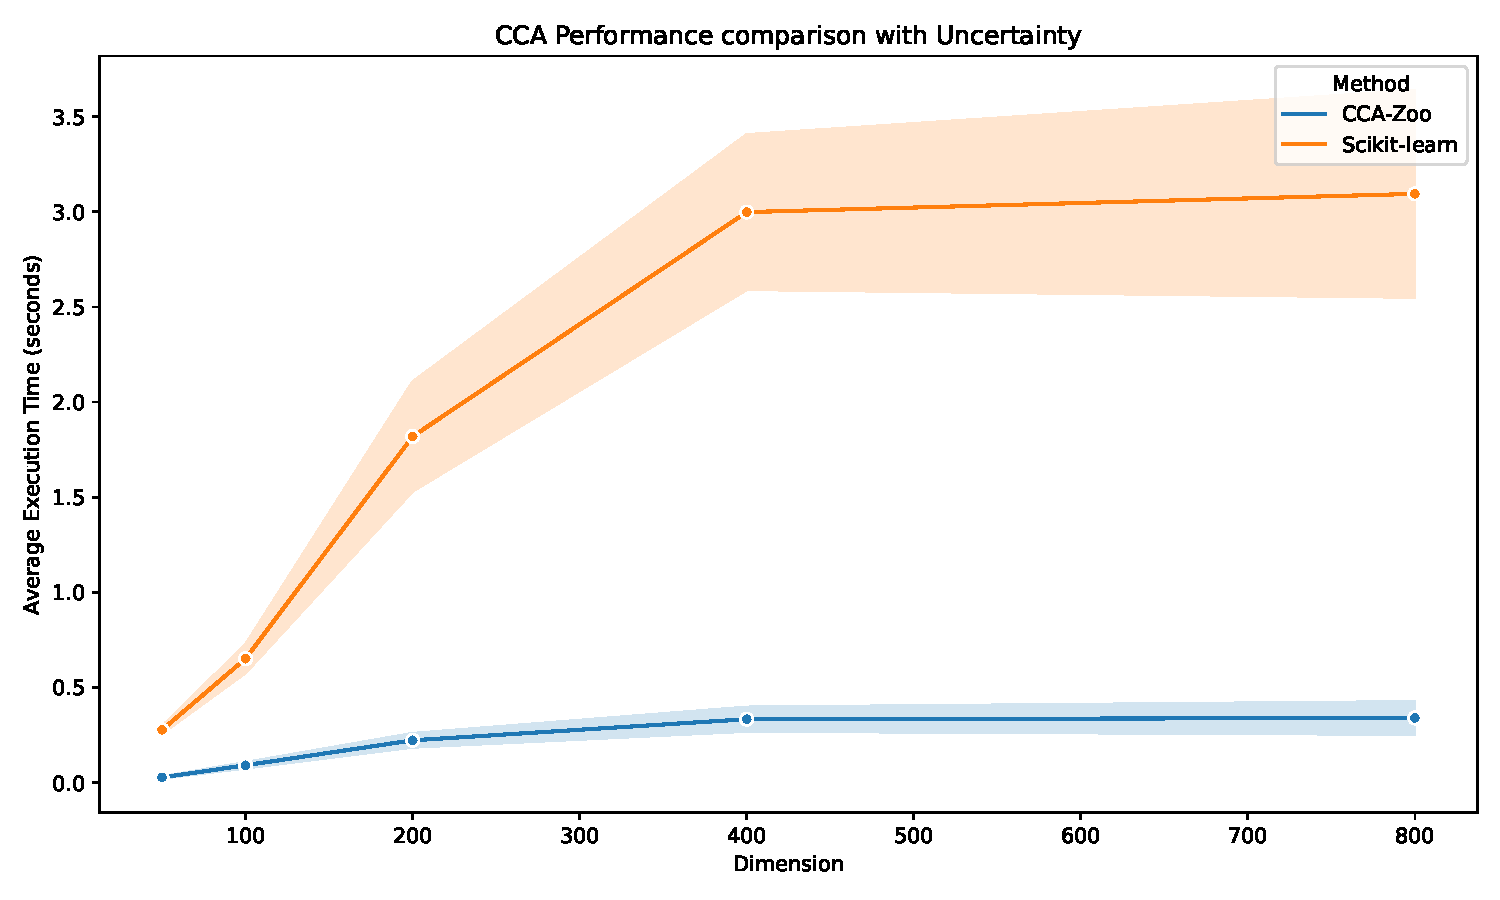
\includegraphics[width=0.8\textwidth]{figures/CCA_Speed_Benchmark}
\caption{Performance comparison for CCA methods}
\label{fig:cca_benchmark}
\end{figure}

\paragraph{Partial Least Squares:}
The comparison for Partial Least Squares is shown in Figure \ref{fig:pls_benchmark}.
Like the CCA experiment, \texttt{CCA-Zoo} maintains a robust performance profile that is competitive with \texttt{scikit-learn}.

\begin{figure}[h]
\centering
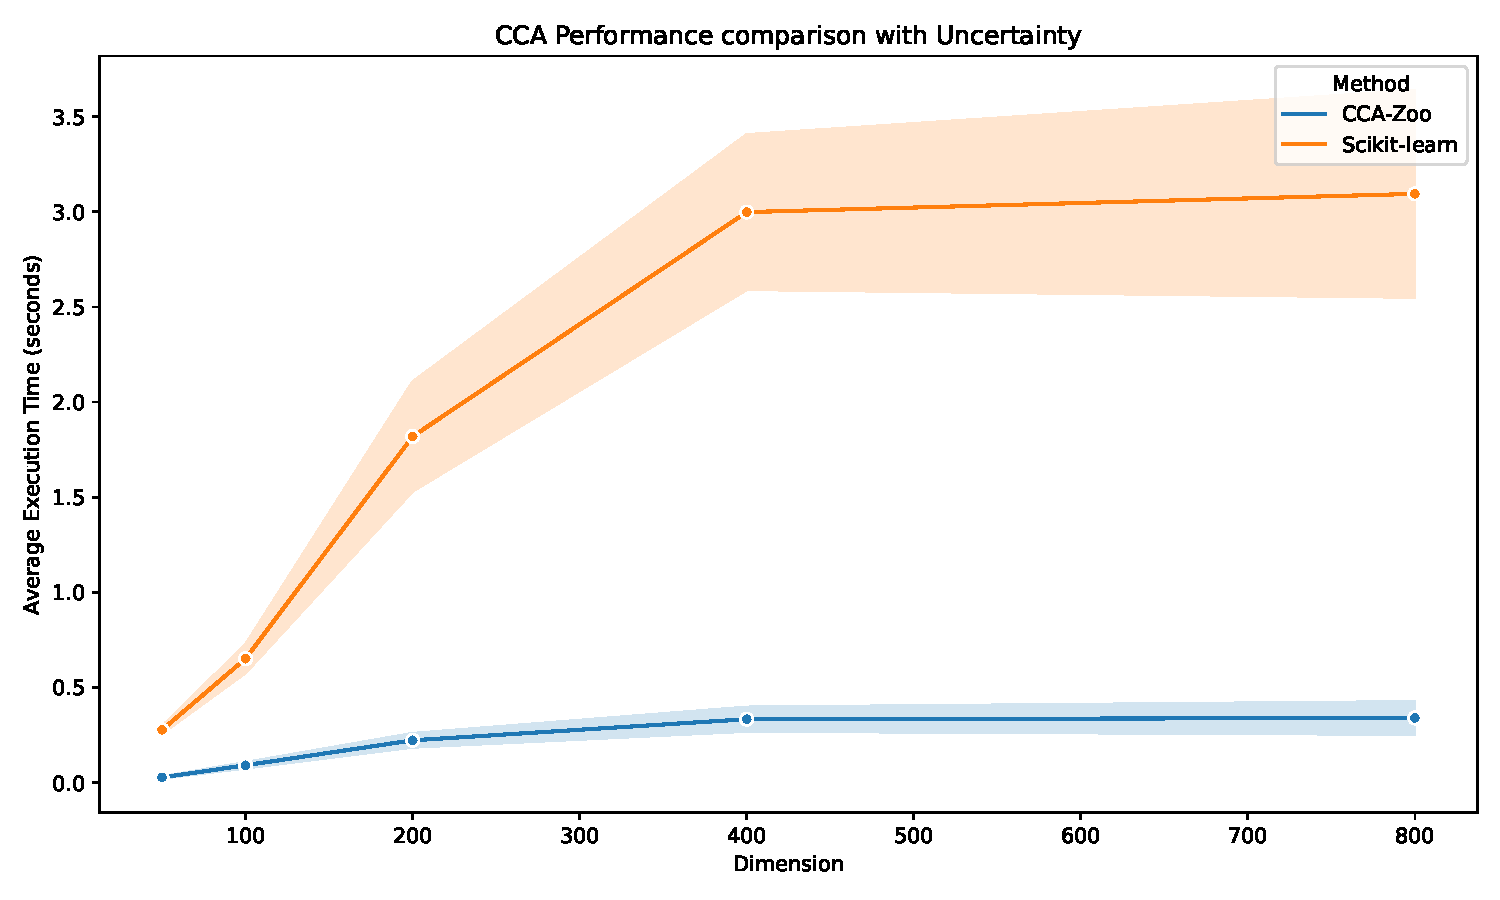
\includegraphics[width=0.8\textwidth]{figures/CCA_Speed_Benchmark}
\caption{Performance comparison for PLS methods}
\label{fig:pls_benchmark}
\end{figure}

\subsubsection{Discussion}

The results indicate that \texttt{CCA-Zoo} is an efficient Python package for both CCA and PLS methods, holding its own against the widely-used \texttt{scikit-learn} library.
These experiments underscore the capability of \texttt{CCA-Zoo} to handle high-dimensional data efficiently, making it a suitable choice for applications in bioinformatics, natural language processing, and other high-dimensional data domains.



\subsection{Experiment 2: Using CCA-Zoo for Brain-Behaviour Association Discovery}

\subsection{Conclusion}

\texttt{CCA-Zoo} has not only served as a tool for my research but aims to be a community resource that can accelerate research and application in multiview learning.
Its design decisions, such as API compatibility and focus on both linear and deep models, reflect a comprehensive understanding of the challenges and opportunities in this field.
